\documentclass[conference]{IEEEtran}
\IEEEoverridecommandlockouts

\usepackage{cite}
\usepackage{amsmath,amssymb,amsfonts}
\usepackage{graphicx}
\usepackage{booktabs}
\usepackage{url}
\usepackage{xcolor}

\begin{document}

\title{Running AEIC: Ultra-Low Bitrate Perceptual Image Compression with a Shallow Encoder on ImageNet-1k}

\author{\IEEEauthorblockN{Benjamin Had\v{z}ihasanovi\'{c}}
\IEEEauthorblockA{Multimedia Systems course project\\
benjaminhadzihasanovic@gmail.com}
\and
\IEEEauthorblockN{Tarik \v{C}aluk}
\IEEEauthorblockA{Multimedia Systems course project}}

\maketitle

\begin{abstract}
This report reproduces the inference pipeline of \emph{Ultra-Low Bitrate Perceptual Image
Compression with Shallow Encoder} (AEIC, CVPR 2026) and evaluates it on a subset of the
ImageNet-1k validation set, a dataset not covered in the original paper. The official PyTorch
implementation was adapted to run on Google Colab: dependency versions were reconciled with the
Colab environment, the C++ entropy-coding engine was made optional for likelihood-based bitrate
estimation, and the evaluation protocol of the authors (bpp, PSNR, MS-SSIM, LPIPS, DISTS, FID,
KID) was applied unchanged. We report rate--distortion--perception results of the shallow-encoder
variant AEIC-SE at five bitrate points below 0.05\,bpp, compare them with the numbers the authors
report on Kodak, DIV2K and CLIC\,2020, and discuss the behaviour of the codec on small,
heterogeneous ImageNet images.
\end{abstract}

\begin{IEEEkeywords}
learned image compression, ultra-low bitrate, diffusion models, perceptual quality, ImageNet
\end{IEEEkeywords}

\section{Problem Statement}
Classical and learned image codecs degrade ungracefully below roughly 0.1 bits per pixel (bpp):
block artifacts, blur, and loss of texture make reconstructions unusable. \emph{Generative} or
\emph{perceptual} codecs address this by allowing the decoder to synthesize plausible detail, so
that reconstructions remain visually convincing even at \emph{ultra-low} bitrates
($<0.05$\,bpp)~\cite{aeic}. Such bitrates matter for bandwidth-constrained links (satellite,
IoT uplinks, disaster communication) where the \emph{sender} is typically a weak edge device.

The problem the paper tackles is the asymmetry of this setting: prior ultra-low bitrate codecs
(e.g., PerCo~\cite{perco}, DiffEIC~\cite{diffeic}, StableCodec~\cite{stablecodec}) push large
pretrained networks --- VAE encoders or tokenizers of latent diffusion models --- onto the
\emph{encoder} side, which contradicts the deployment reality that the encoder runs on the weak
device while the decoder (cloud, workstation) can be heavy. AEIC asks: \emph{how simple can the
encoder become at ultra-low bitrates without sacrificing decoded quality?} The paper's key
observation is that as the rate $\mathcal{R}$ decreases, the information the encoder must extract
shrinks, so encoding complexity can be reduced drastically; the heavy generative lifting is moved
entirely to the decoder.

\section{The AEIC Algorithm}
\subsection{Asymmetric architecture}
AEIC (Asymmetric Extreme Image Compression) is a variational compression model with three parts:

\textbf{Shallow analysis transform (encoder).} A small StarNet-style convolutional network
$g_a$ maps the RGB image directly (no VAE) to a compact latent $y$ with $32\times$ spatial
downsampling. Two variants are provided: \mbox{AEIC-ME} (``moderate'': 2 blocks per stage,
widths 64--320, 3.09\,M parameters, 204\,KMACs/pixel) and \mbox{AEIC-SE} (``shallow'': 1 block
per stage, widths 32--256, 0.94\,M parameters, 46\,KMACs/pixel). The shallow variant encodes
1080p images at 35.8\,FPS --- an $\sim$18--19$\times$ encoding speed-up over StableCodec and
DLF~\cite{aeic}.

\textbf{Entropy model.} A scale--mean hyperprior~\cite{balle} with a quadtree-partition spatial
context model: the latent is split into four interleaved groups that are coded sequentially, each
group's Gaussian parameters $(\mu,\sigma)$ being predicted from the hyper-latent $\hat z$ and the
already-decoded groups. Latents are quantized by rounding to the predicted mean and
entropy-coded with rANS.

\textbf{One-step diffusion decoder.} The decoded latent is mapped by a synthesis transform into
the latent space of SD-Turbo~\cite{sdturbo}; a LoRA-adapted (rank 32) SD-Turbo UNet performs a
\emph{single} denoising step (plus a residual skip path that preserves structure), and a pruned
``half'' VAE decoder~\cite{adcsr} produces the image. One-step denoising keeps decoding latency
comparable to GAN decoders while retaining diffusion-prior texture synthesis.

\subsection{Dual-side feature distillation}
To close the quality gap between the shallow and the moderate encoder, AEIC-SE is trained with
knowledge distillation from AEIC-ME on both sides of the pipeline: an \emph{encoder-side} loss
aligns the latent $y$, hyper-latent $z$, quantized latent $\hat y$, and decoded features through
learned $1\times1$ projection layers; a \emph{decoder-side} loss matches the diffusion input
latents, the UNet output, and intermediate UNet feature maps. The paper's ablation shows that
without distillation AEIC-SE loses 8.5\% LPIPS / 23.8\% DISTS relative to AEIC-ME, while with
both losses the gap shrinks below 3\%~\cite{aeic}.

\subsection{Training}
Training has three stages (we did \emph{not} retrain; listed for completeness):
(1) 300k iterations at a relaxed rate target with MSE + LPIPS + semantic distortion;
(2) 30k iterations pushed to the ultra-low rate target, adding a DINOv3-based adversarial loss
and overlapped-chunk DISTS;
(3) for AEIC-SE, 5k iterations of high-resolution ($1024^2$) fine-tuning.
The released checkpoints \texttt{ft2}--\texttt{ft32} correspond to five rate--lambda settings
spanning roughly 0.004--0.037\,bpp.

\section{Our Implementation}
\subsection{Setup}
We used the official repository\footnote{\url{https://github.com/LuizScarlet/AEIC}} with the
released pretrained checkpoints and ran all experiments on Google Colab (NVIDIA T4, 16\,GB).
Our notebook performs the full pipeline: environment setup, model download (SD-Turbo VAE+UNet,
pruned VAE decoder, five AEIC-SE checkpoints), dataset preparation, compression, and evaluation
with the authors' \texttt{evaluate.py} (itself adapted from MS-ILLM~\cite{msillm}, so the metric
implementations match the paper).

\subsection{ImageNet-1k data}
The paper evaluates on Kodak, DIV2K and CLIC\,2020; our task was to run the codec on
ImageNet-1k~\cite{imagenet}. We streamed the official validation split from Hugging Face and
exported the first $N{=}500$ images whose shorter side is at least 256\,px as lossless
PNG (the repository's I/O expects PNG). The size filter is needed because MS-SSIM requires
inputs larger than $\sim$160\,px after its four dyadic downsamplings, and it mirrors the paper's
full-resolution protocol --- images are compressed at their native resolution, with internal
reflection padding to multiples of 64.

\subsection{Modifications to the original code}
Only five small changes were required ("slight modification" as anticipated by the assignment):
\begin{enumerate}
\item \textbf{Optional entropy-coding engine.} \texttt{compress.py} unconditionally builds rANS
CDF tables, which requires compiling the repo's C++/pybind11 engine. Since AEIC also reports the
bitrate estimated from the entropy model's likelihoods, we guarded this call behind the
\texttt{--use\_practical\_entropy\_coding} flag. We separately built the C++ engine and verified
real bitstream sizes against the estimate at the \texttt{ft8} rate point: 0.0180\,bpp on a
50-image subset vs.\ 0.0167\,bpp estimated over the full set --- a ${\approx}7\%$ gap consistent
with the per-image header and rANS overhead, which weigh more on small images.
\item \textbf{Attention backend.} xformers (pinned to an old PyTorch) was replaced by PyTorch's
built-in scaled-dot-product attention by defaulting the xformers flag to off.
\item \textbf{No \texttt{torch.compile}.} ImageNet images have varying resolutions, so
compilation would be re-triggered for nearly every input shape; we disabled the
\texttt{compile\_model} default.
\item \textbf{Local patch-FID implementation.} \texttt{evaluate.py} imports
\texttt{update\_patch\_fid} from the \texttt{neuralcompression} package, which no longer builds
in the Colab environment (its \texttt{compressai} dependency fails to compile). As it is the only
function used, we replaced it with a faithful local port of the ``FID/256'' protocol of Mentzer
et al.: non-overlapping $256^2$ patches plus a second, half-patch-offset pass for images larger
than $1.5\times$ the patch size, converted to 8-bit before updating the FID/KID statistics.
\item \textbf{KID subset size.} ImageNet images yield only 1--2 patches of $256^2$ each, so the
KID default \texttt{subset\_size}=1000 can exceed the total patch count and abort the
computation; we lowered it to 50, which changes only the variance of the unbiased KID estimate,
not its expectation.
\end{enumerate}
In addition, library versions had to be reconciled: the model code imports module paths that
moved after \texttt{diffusers} 0.25, so we pinned \texttt{diffusers==0.25.1},
\texttt{transformers==4.46.3}, \texttt{huggingface\_hub==0.25.0} and \texttt{peft==0.13.2} while
keeping Colab's preinstalled PyTorch.

\section{Metrics}
All metrics are those used in the paper, computed by the authors' script:
\begin{itemize}
\item \textbf{bpp} (bits per pixel): compressed size divided by pixel count --- the \emph{rate}.
\item \textbf{PSNR} (dB, $\uparrow$): log inverse MSE; pixel-exact fidelity. At ultra-low rates
generative codecs deliberately sacrifice PSNR for realism.
\item \textbf{MS-SSIM} ($\uparrow$): multi-scale structural similarity; correlates with perceived
structural fidelity better than PSNR.
\item \textbf{LPIPS} ($\downarrow$)~\cite{lpips}: distance between AlexNet features of the two
images; measures perceptual similarity to the \emph{specific} original.
\item \textbf{DISTS} ($\downarrow$)~\cite{dists}: combines deep structure and texture similarity;
more tolerant to resampled textures, which suits generative codecs.
\item \textbf{FID} ($\downarrow$)~\cite{fid} / \textbf{KID} ($\downarrow$)~\cite{kid}: distance
between Inception feature \emph{distributions} of originals and reconstructions (computed
patch-wise as in MS-ILLM); they measure realism without requiring per-pixel alignment.
\end{itemize}
Together they cover the rate--distortion--perception trade-off: PSNR/MS-SSIM measure distortion,
LPIPS/DISTS perceptual similarity, FID/KID statistical realism.

\section{Problems Faced and Solutions}
\begin{enumerate}
\item \textbf{Dependency conflicts.} The repo pins \texttt{torch==2.1.2} and old CUDA libraries
that clash with Colab, and its \texttt{neuralcompression} dependency fails to build there
entirely (compilation error in \texttt{compressai}), which aborts the whole pinned install.
Solution: keep Colab's PyTorch, pin only the libraries whose APIs the code actually relies on
(diffusers/transformers/hub/peft), drop \texttt{neuralcompression} in favour of the local
patch-FID port (Sec.~III-C), and disable xformers (see above).
\item \textbf{Gated ImageNet access.} \texttt{ILSVRC/imagenet-1k} on Hugging Face requires
accepting the ImageNet license. Solution: stream with a user token after accepting the terms; an
ungated mirror of the validation split is used as fallback. Streaming avoids downloading the full
6.7\,GB split for a 500-image subset.
\item \textbf{C++ entropy coder on Colab.} Building cmake projects inside a notebook is fragile
and unnecessary for likelihood-based bpp; moreover, the build fetches pybind11 v2.10.4, which
predates Colab's Python 3.12 and fails to compile the rANS bindings (while, confusingly, the
simpler CDF module builds fine). Solution: the one-line guard described in Sec.~III-C for the
main pipeline, and for the verification build a bump of the fetched pybind11 to v2.13.6 plus
removal of the \texttt{-Werror} flag that recent g++ warnings would otherwise trip.
\item \textbf{Variable image sizes.} \texttt{torch.compile} recompilation (disabled) and MS-SSIM
minimum-size constraints (handled by the 256\,px filter). Reflection padding to multiples of 64
also means small images carry proportionally more padded content, which inflates bpp slightly
compared to 2K test sets.
\item \textbf{Colab session limits.} A full run (5 checkpoints $\times$ 500 images plus metric
networks) takes 2--2.5\,h on a T4. Solution: per-checkpoint logs and outputs are persisted, so an
interrupted run only needs the missing checkpoints repeated.
\end{enumerate}

\section{Results and Interpretation}
Table~\ref{tab:results} reports our measurements on the ImageNet-1k validation subset;
Fig.~\ref{fig:rd} shows the rate--metric curves against the values the authors report on Kodak
and CLIC\,2020 (from \texttt{results/} in the repo). Fig.~\ref{fig:sweep} traces two examples
across the full rate sweep and Fig.~\ref{fig:qual} shows further qualitative examples. As a
classical reference we additionally encoded the same 500 images with JPEG at its \emph{minimum}
quality setting (Pillow/libjpeg, quality 1) and evaluated identically (last row of
Table~\ref{tab:results}).

\begin{table}[t]
\caption{AEIC-SE on 500 ImageNet-1k validation images (shorter side $\geq$ 256\,px), ordered by
increasing bitrate, plus a JPEG baseline at its lowest quality setting. PSNR in dB; KID is the
mean of the unbiased estimate (subset size 50).}
\label{tab:results}
\centering
\small
\begin{tabular}{lccccccc}
\toprule
ckpt & bpp & PSNR & MS-SSIM & LPIPS & DISTS & FID & KID \\
\midrule
ft32 & 0.0049 & 17.71 & 0.576 & 0.374 & 0.202 & 60.1 & 0.0064 \\
ft16 & 0.0093 & 18.86 & 0.657 & 0.299 & 0.169 & 48.4 & 0.0029 \\
ft8  & 0.0167 & 19.99 & 0.728 & 0.237 & 0.144 & 39.6 & 0.0015 \\
ft4  & 0.0282 & 20.97 & 0.786 & 0.190 & 0.122 & 31.5 & 0.0006 \\
ft2  & 0.0431 & 21.75 & 0.825 & 0.157 & 0.106 & 26.5 & $-0.0002$ \\
\midrule
JPEG$_{q=1}$ & 0.1915 & 21.07 & 0.809 & 0.547 & 0.411 & 151.5 & 0.0651 \\
\bottomrule
\end{tabular}
\end{table}

\begin{figure}[t]
\centering
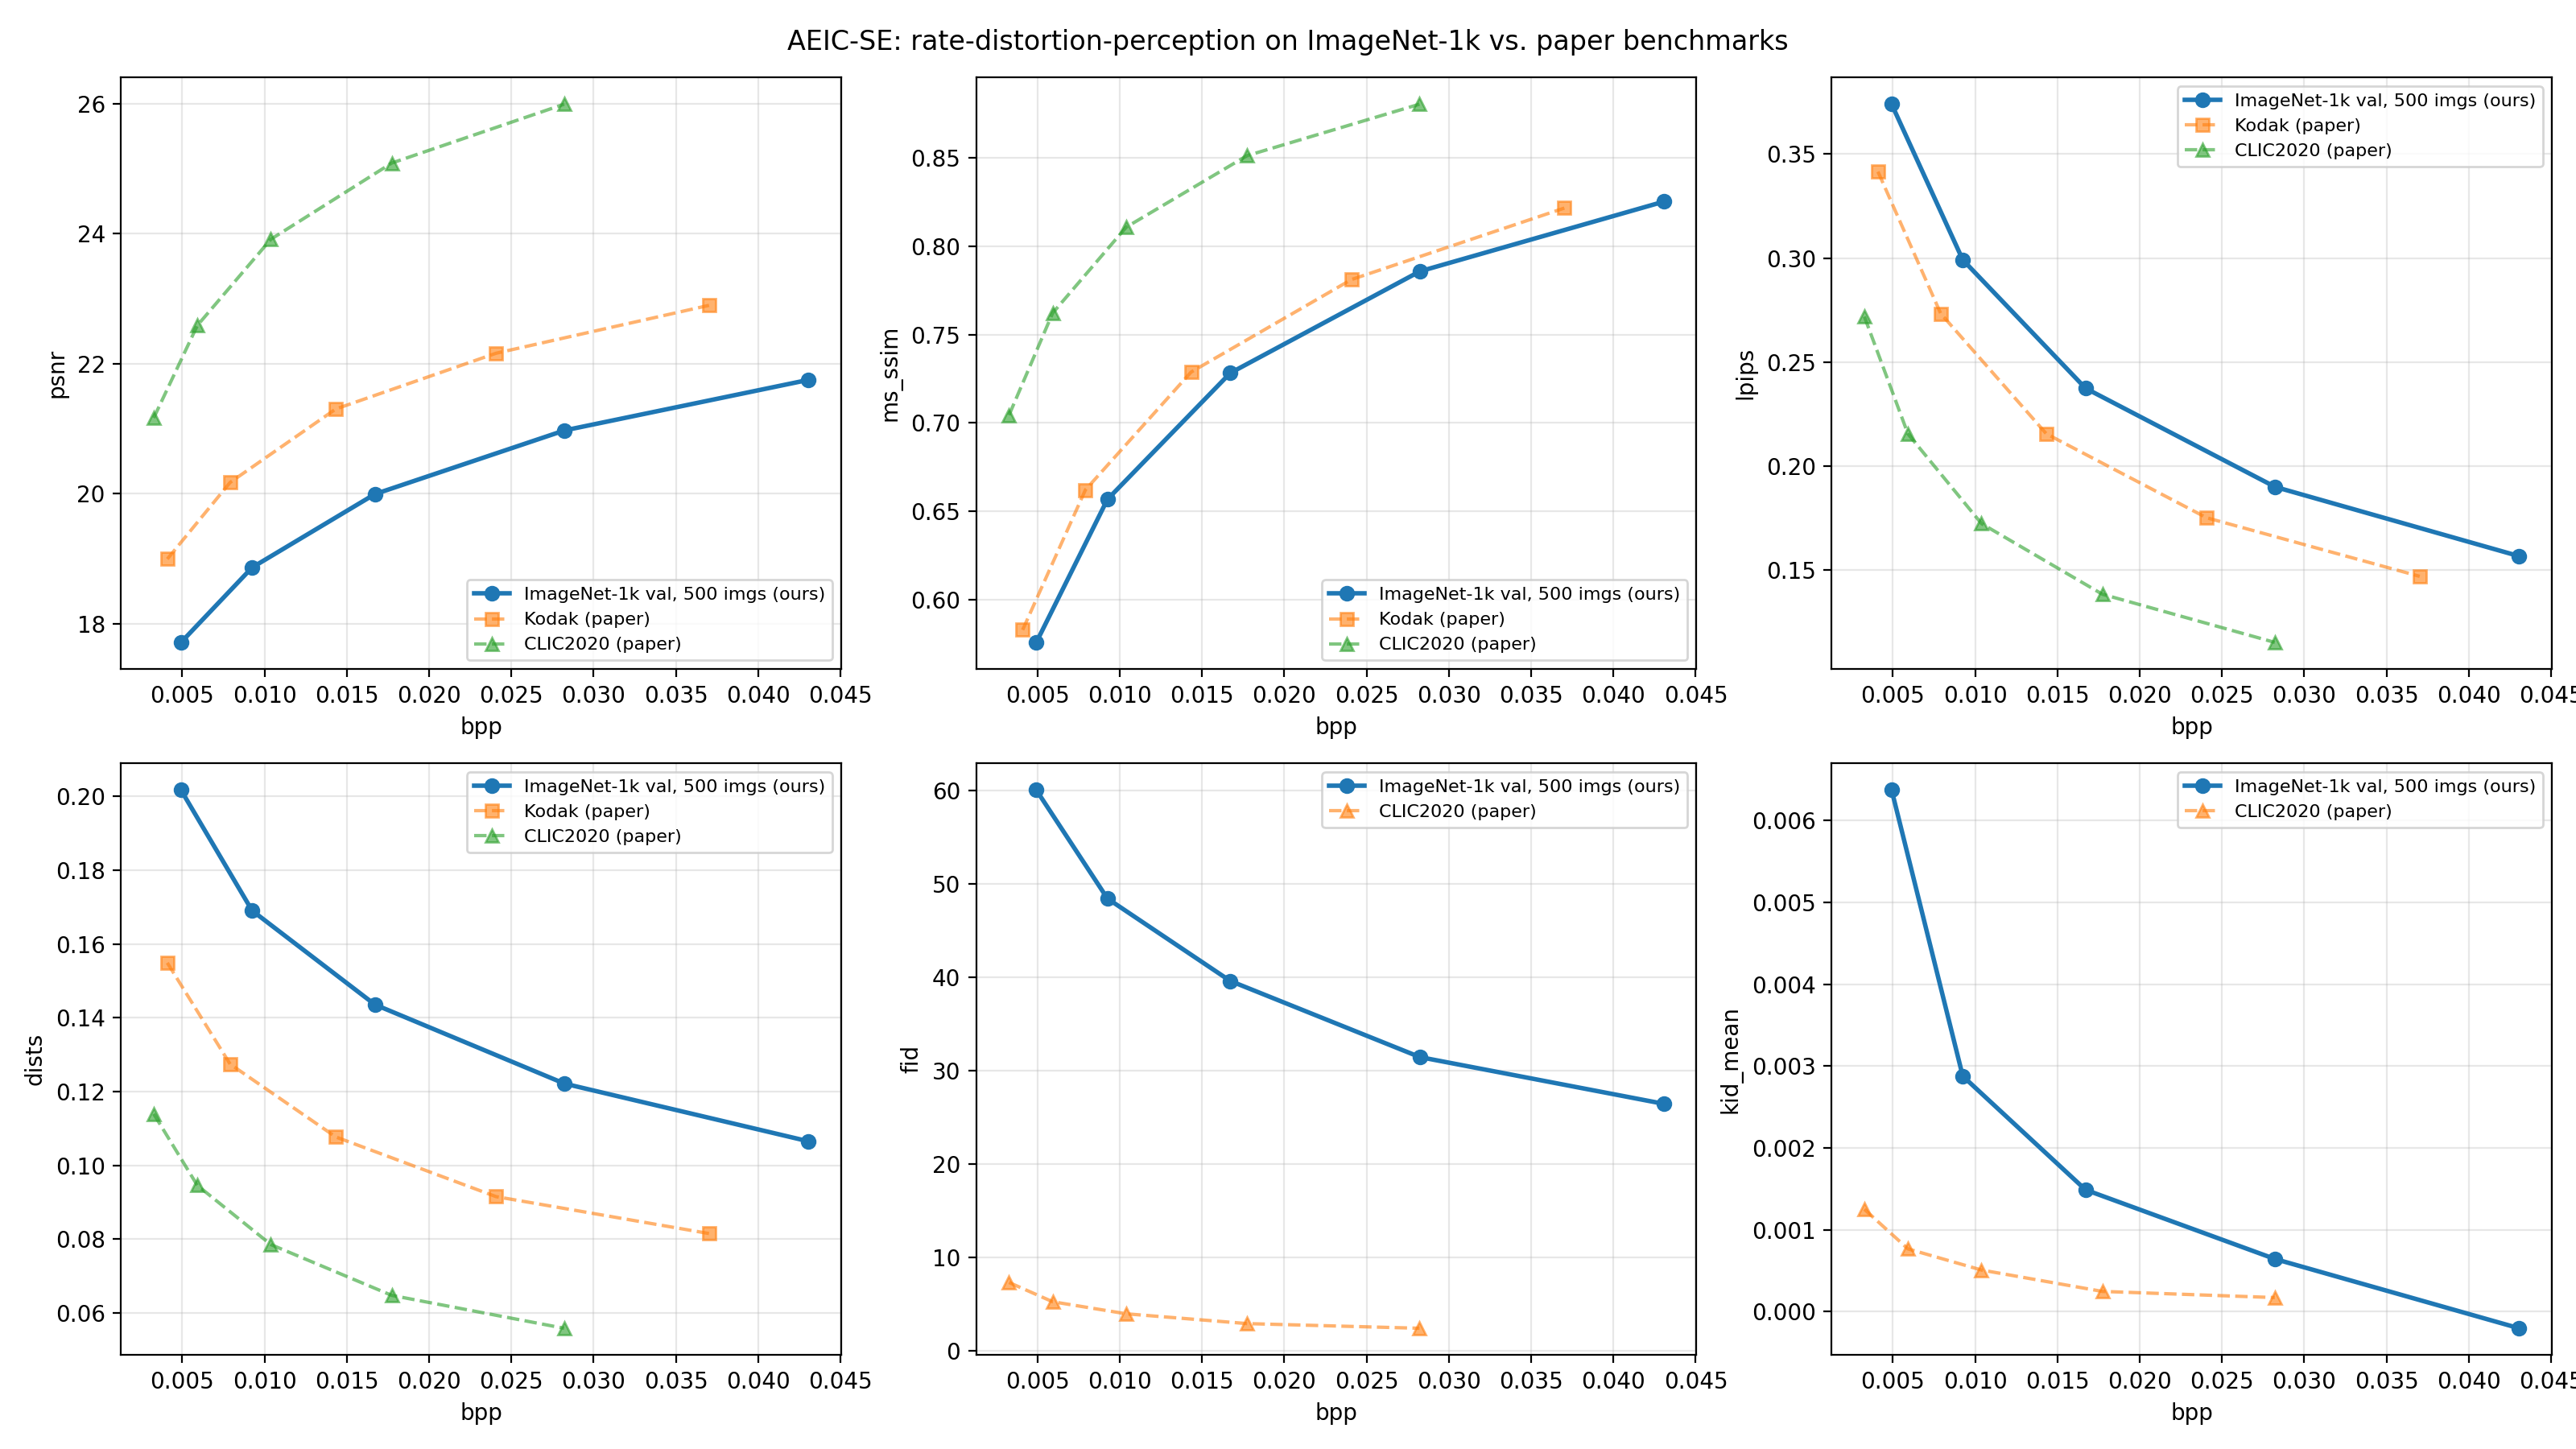
\includegraphics[width=\linewidth]{rd_curves_imagenet.png}
\caption{Rate--distortion--perception curves of AEIC-SE on ImageNet-1k (ours) vs.\ the authors'
Kodak and CLIC\,2020 results.}
\label{fig:rd}
\end{figure}

\begin{figure*}[t]
\centering
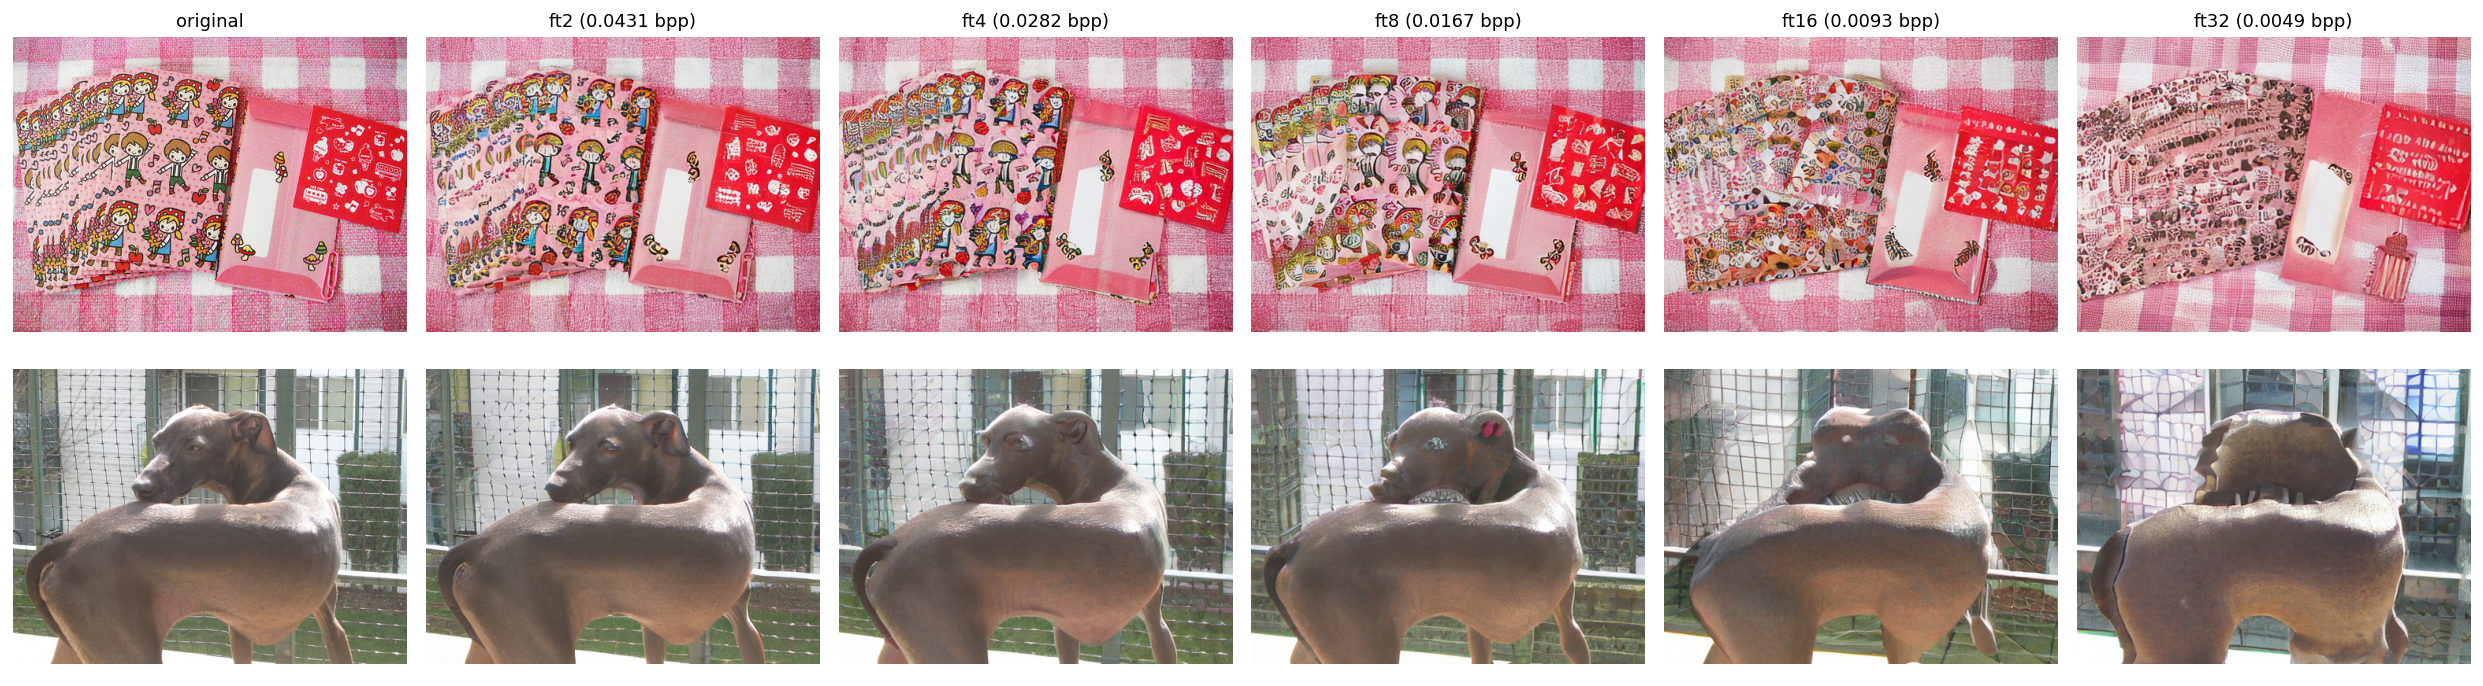
\includegraphics[width=\textwidth]{rate_sweep_imagenet.png}
\caption{Two validation images across the full rate sweep (original, then highest to lowest
bitrate). Degradation is gradual and content-dependent: fine repetitive detail and printed text
(top) are re-synthesized increasingly loosely as the rate drops, while in the bottom row the
animal's fur and the thin wire fence stay plausible down to \texttt{ft16} (0.009\,bpp) but are
visibly redrawn at \texttt{ft32} (0.005\,bpp) --- content classes (text, regular thin
structures) where generative hallucination is most critical.}
\label{fig:sweep}
\end{figure*}

\begin{figure}[t]
\centering
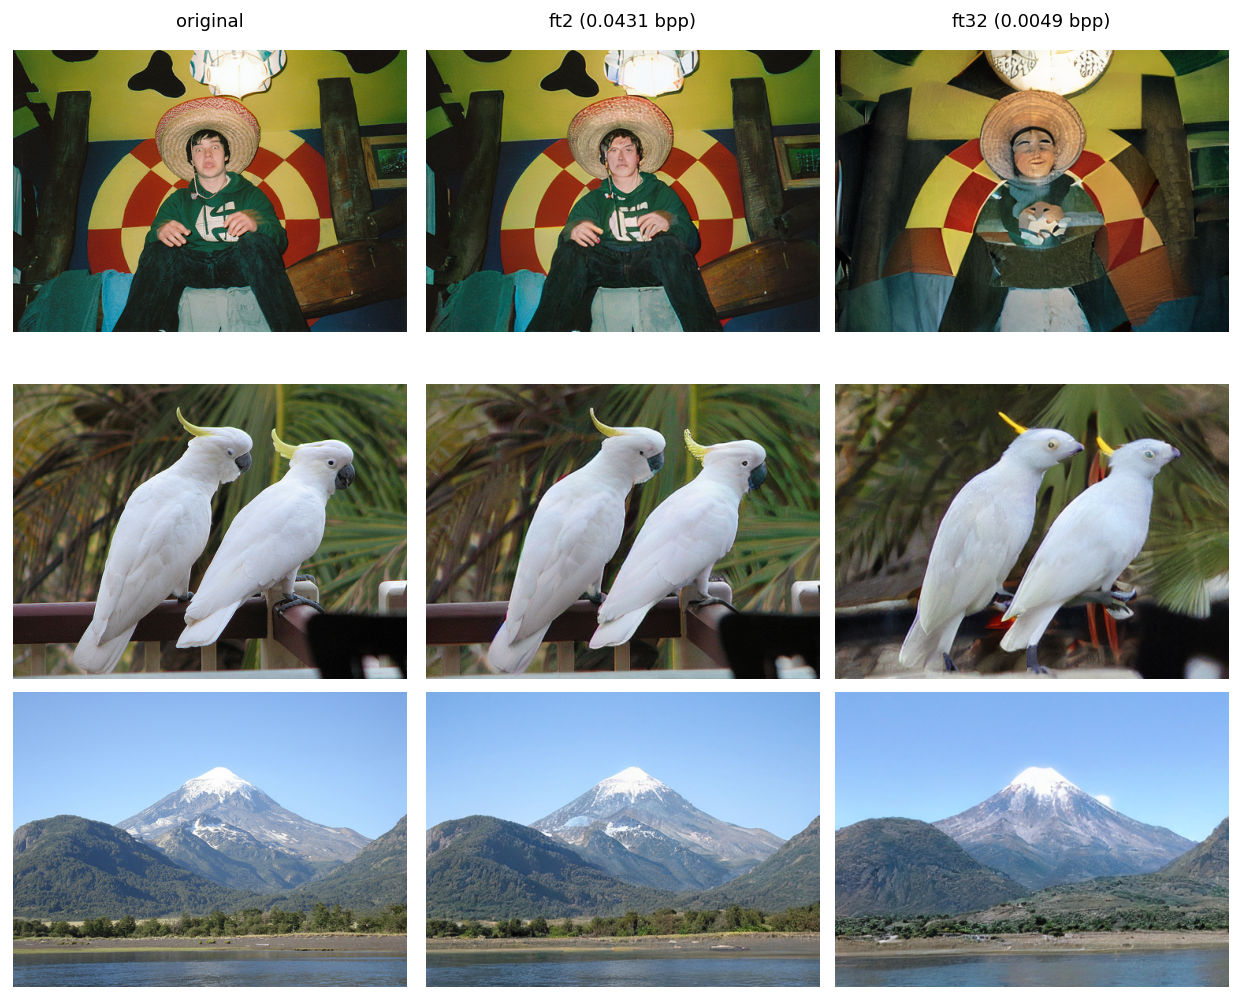
\includegraphics[width=\linewidth]{qualitative_imagenet.png}
\caption{Original vs.\ reconstructions at the highest (\texttt{ft2}, 0.043\,bpp) and lowest
(\texttt{ft32}, 0.005\,bpp) released rate points, on three further validation images.}
\label{fig:qual}
\end{figure}

Our observations:
\begin{itemize}
\item \textbf{Consistent trade-off shape.} All seven metrics improve monotonically with rate
across the full span (0.0049--0.0431\,bpp), tracing the same curve shapes as the paper's
benchmarks --- the codec generalizes to a dataset it was never trained or tested on.
\item \textbf{Small-image rate overhead.} At a given checkpoint the bitrate is roughly 50\%
higher than the authors measure on CLIC\,2020 (e.g., 0.0049 vs.\ 0.0033\,bpp at the lowest
point). ImageNet images are small ($\sim$0.2\,MP vs.\ $\sim$4\,MP), so the constant hyper-latent
cost and the padding to multiples of 64 are amortized over far fewer pixels.
\item \textbf{Fidelity close to Kodak.} MS-SSIM (0.576--0.825) almost coincides with the
authors' Kodak range (0.583--0.822); PSNR is about 1\,dB lower and LPIPS/DISTS moderately worse
at matched rates. This fits ImageNet's much higher content diversity --- and the fact that
ImageNet ``originals'' are themselves JPEGs, so the ground truth already contains compression
artifacts that the codec has no reason to reproduce.
\item \textbf{Classical coding cannot reach this regime.} JPEG at its lowest quality setting
still spends 0.19\,bpp --- $4.4\times$ the bits of \texttt{ft2} and $39\times$ those of
\texttt{ft32} --- so bitrates below 0.05\,bpp are simply unreachable for it. Moreover, despite
comparable pixel fidelity (PSNR 21.1\,dB, MS-SSIM 0.809, close to \texttt{ft2}), JPEG is
drastically worse on every perceptual metric: LPIPS 0.547 vs.\ 0.157, DISTS 0.411 vs.\ 0.106,
FID 151.5 vs.\ 26.5. This is the clearest illustration in our study of why PSNR alone is a
misleading objective at extreme rates, and of the advantage of generative compression.
\item \textbf{Subjective quality.} Visual inspection of side-by-side sheets
(Fig.~\ref{fig:sweep}) matches the metrics: down to \texttt{ft16} (0.009\,bpp) reconstructions
are hard to distinguish from the original at normal viewing distance, with differences emerging
only when zooming into fine texture; at \texttt{ft32} (0.005\,bpp), hallucinated textures and
altered object details are evident at any viewing distance. For untargeted browsing-grade use,
the practical operating point of AEIC-SE on ImageNet-sized images thus lies around
0.01--0.02\,bpp.
\item \textbf{FID/KID need careful reading.} Absolute FID (26.5--60.1) is an order of magnitude
above the CLIC values (2.5--7.4). This is expected: small images contribute only 1--2 patches of
$256^2$ each, so the statistic is built from $\sim$600 patches instead of $\sim$20\,000, and FID
is strongly biased upward at small sample sizes; the ImageNet distribution is also far more
diverse. The monotonic trend is the meaningful signal. Notably, KID --- which is unbiased --- is
slightly \emph{negative} at the highest rate ($-2\times10^{-4} \pm 1.9\times10^{-3}$), i.e.,
statistically indistinguishable from zero: at 0.043\,bpp the reconstructed patch distribution
cannot be told apart from the original one at this sample size.
\end{itemize}

\section{Possible Improvements}
\begin{itemize}
\item \textbf{Resolution-adaptive signalling.} Reduce the fixed per-image overhead (hyper-latent,
padding) that penalizes small images, e.g., content-adaptive padding or a hyper-latent whose
footprint scales with image entropy.
\item \textbf{Single variable-rate model.} The five released checkpoints could be folded into one
model conditioned on a rate token, removing the need to ship multiple weights.
\item \textbf{Even lighter decoding.} Distill the one-step SD-Turbo UNet into a smaller student
to allow ultra-low bitrate decoding on mid-range devices, not only encoding.
\item \textbf{Semantic bit allocation.} Steer bits toward salient regions (faces, text) where
generative hallucination is risky; text and faces are the typical failure cases at these rates.
\item \textbf{Fidelity control.} A user-tunable distortion/realism knob (e.g., guidance on the
residual branch) would let applications choose between pixel faithfulness and texture realism.
\item \textbf{Video extension.} The shallow-encoder argument applies even more to video uplinks;
temporal context could further cut the rate.
\end{itemize}

\section{Conclusion}
The official AEIC implementation runs on ImageNet-1k after only minor, well-understood
modifications. The shallow-encoder variant maintains the paper's rate--distortion--perception
behaviour on a dataset it was never tuned on, supporting the paper's central claim that at
ultra-low bitrates the encoder can be made very cheap while a one-step diffusion decoder
preserves perceptual quality. A JPEG reference at its quality floor needs over four times the
bits of the highest AEIC rate point while scoring drastically worse on all perceptual metrics,
underlining why generative codecs are the only practical option in this regime.

\begin{thebibliography}{00}
\bibitem{aeic} T. Zhang, D. Liu, and C. W. Chen, ``Ultra-low bitrate perceptual image
compression with shallow encoder,'' in \emph{Proc. IEEE/CVF CVPR}, 2026, arXiv:2512.12229.
\bibitem{stablecodec} T. Zhang, X. Luo, L. Li, and D. Liu, ``StableCodec: Taming one-step
diffusion for extreme image compression,'' in \emph{Proc. IEEE/CVF ICCV}, 2025.
\bibitem{perco} M. Careil, M. J. Muckley, J. Verbeek, and S. Lathuili\`ere, ``Towards image
compression with perfect realism at ultra-low bitrates,'' in \emph{Proc. ICLR}, 2024.
\bibitem{diffeic} Z. Li et al., ``Towards extreme image compression with latent feature guidance
and diffusion prior,'' \emph{IEEE TCSVT}, 2024.
\bibitem{balle} J. Ball\'e, D. Minnen, S. Singh, S. J. Hwang, and N. Johnston, ``Variational
image compression with a scale hyperprior,'' in \emph{Proc. ICLR}, 2018.
\bibitem{sdturbo} A. Sauer, D. Lorenz, A. Blattmann, and R. Rombach, ``Adversarial diffusion
distillation,'' in \emph{Proc. ECCV}, 2024.
\bibitem{adcsr} H. Chen et al., ``Adversarial diffusion compression for real-world image
super-resolution,'' in \emph{Proc. IEEE/CVF CVPR}, 2025.
\bibitem{msillm} M. J. Muckley, A. El-Nouby, K. Ullrich, H. J\'egou, and J. Verbeek, ``Improving
statistical fidelity for neural image compression with implicit local likelihood models,'' in
\emph{Proc. ICML}, 2023.
\bibitem{imagenet} O. Russakovsky et al., ``ImageNet large scale visual recognition challenge,''
\emph{IJCV}, vol. 115, no. 3, pp. 211--252, 2015.
\bibitem{lpips} R. Zhang, P. Isola, A. A. Efros, E. Shechtman, and O. Wang, ``The unreasonable
effectiveness of deep features as a perceptual metric,'' in \emph{Proc. IEEE/CVF CVPR}, 2018.
\bibitem{dists} K. Ding, K. Ma, S. Wang, and E. P. Simoncelli, ``Image quality assessment:
Unifying structure and texture similarity,'' \emph{IEEE TPAMI}, vol. 44, no. 5, 2022.
\bibitem{fid} M. Heusel, H. Ramsauer, T. Unterthiner, B. Nessler, and S. Hochreiter, ``GANs
trained by a two time-scale update rule converge to a local Nash equilibrium,'' in \emph{Proc.
NeurIPS}, 2017.
\bibitem{kid} M. Bi\'nkowski, D. J. Sutherland, M. Arbel, and A. Gretton, ``Demystifying MMD
GANs,'' in \emph{Proc. ICLR}, 2018.
\end{thebibliography}

\end{document}
